\documentclass[twocolumn,11pt]{article}
\setlength{\textheight}{9truein}
\setlength{\topmargin}{-0.9truein}
\setlength{\parindent}{0pt}
\setlength{\parskip}{10pt}
\setlength{\columnsep}{.4in}

\usepackage{amsmath,amsfonts,amssymb,amsthm,bm,caption,calc,ifthen,graphicx,url,hyperref}

\begin{document}
\pagestyle{plain}
\onecolumn
ASTP720 
\newline Homework 5
\newline Will Wainwright
\newline Repository: \href{https://github.com/wjwainwright/ASTP720}{https://github.com/wjwainwright/ASTP720}

\section*{Discussion}
In order to stack the data and fold it to create a phase diagram, I located the lowest point in each transit dip and stacked the data around those points. In order to do this, I therefore considered the lowest point in the dip to be at zero period. I used the gap in time in-between these dips to determine the average period of transit to be 3.548 days, just over 85 hours. I believe the appearance of the stacked points, falling in columns that are evenly spaced, is due to the timing interval at which the data are sampled. In order to determine the rest of the parameters, I used MCMC to fit a box function. My box function is pretty simple. It takes a center position, ad width, and a depth. IF the x point it receives is outside the center $\pm$ half the width, it returns 1. If it is within that range, it returns 1 - depth. I fit an example of this function, using parameters that work well by eye, to the phase diagram in Figure 3. I used these parameters as my initial guess for the MCMC, and ran it for 1000 iterations. The result of the MCMC fitting can be seen in Figure 4. While the center and width values seem to have been accurately determined by the algorithm, for whatever reason the depth that the function returns is highly variable. It can vary from being several times deeper than it should be, to being negative and extending above 1 on the y-axis. Given how close it is to the end of the semester, I do not have time to further investigate this phenomenon. 

My MCMC method stores a list of the current values for all 3 parameters that are being fit. Every iteration, it calculates the current and proposed likelihoods for each variable separately, using last step's values for the two variables that are not being proposed as a baseline. In order to compute the metropolis ratio, I had to use the sum of the log likelihoods, instead of the product of the likelihoods. This is because I was calculating incredibly small numbers that returned 0.0 as a float. Altogether, I would say that I learned a lot about MCMC and it is another tool that I have under my belt, even if it is one I am extremely novice with.

For the purpose of determining the type of planet, I am forced to use an estimate for the fractional dip size, since the MCMC is not working ideally. I believe the dip to be on the order of 0.0075, which means the fractional dip is also 0.0075 since the baseline intensity is 1. This means that the radius of the planet is around 0.155$R_{\odot}$. That makes this planet roughly 1.5 times the radius of Jupiter, with an orbital period more than 1200 times shorter than that of Jupiter. Quite different than our solar system for sure.


\begin{figure}[!h]
	\centering
	\noindent
	\makebox[\textwidth]{
      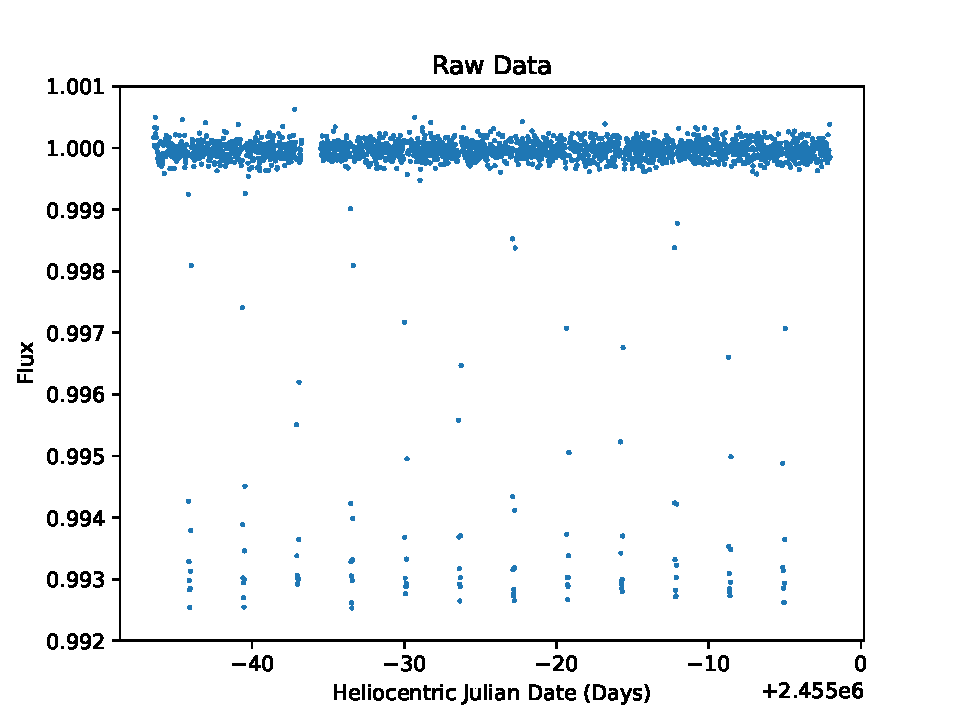
\includegraphics[width=4.5in]{raw.pdf}}
      \caption{Plot of the raw signal data.}
\end{figure}

\begin{figure}[!h]
	\centering
	\noindent
	\makebox[\textwidth]{
      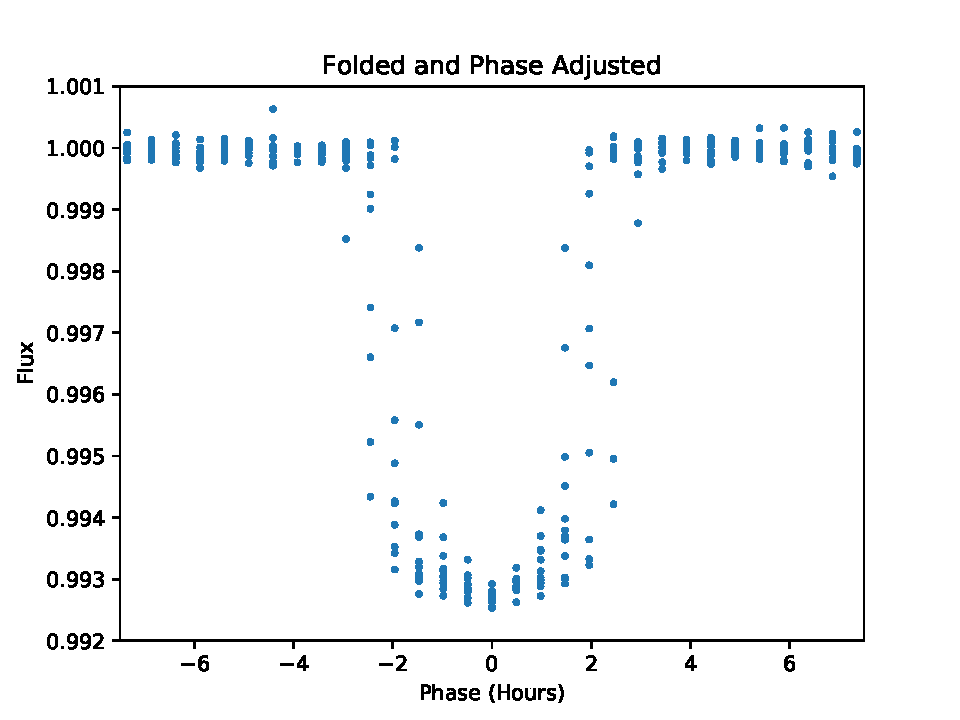
\includegraphics[width=4.5in]{folded.pdf}}
      \caption{Plot of signal having been folded and phased. The minimum point in each transit was used as the zero period marker.}
\end{figure}

\begin{figure}[!h]
	\centering
	\noindent
	\makebox[\textwidth]{
      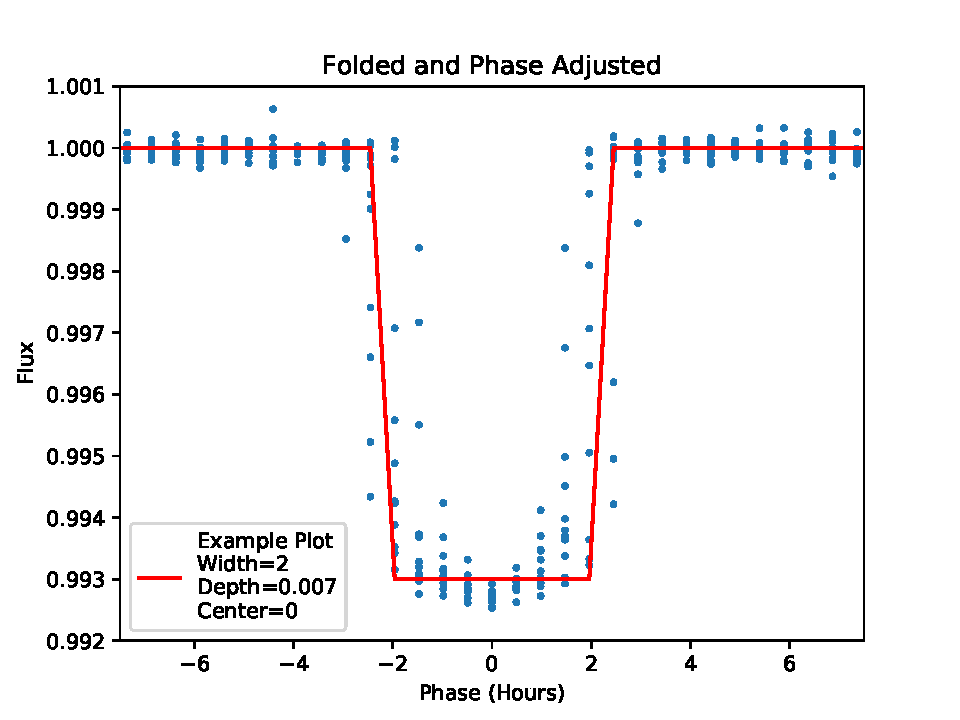
\includegraphics[width=4.5in]{test.pdf}}
      \caption{Plot of signal having been folded and phased. The starting guess parameters for the box plot function are shown.}
\end{figure}

\begin{figure}[!h]
	\centering
	\noindent
	\makebox[\textwidth]{
      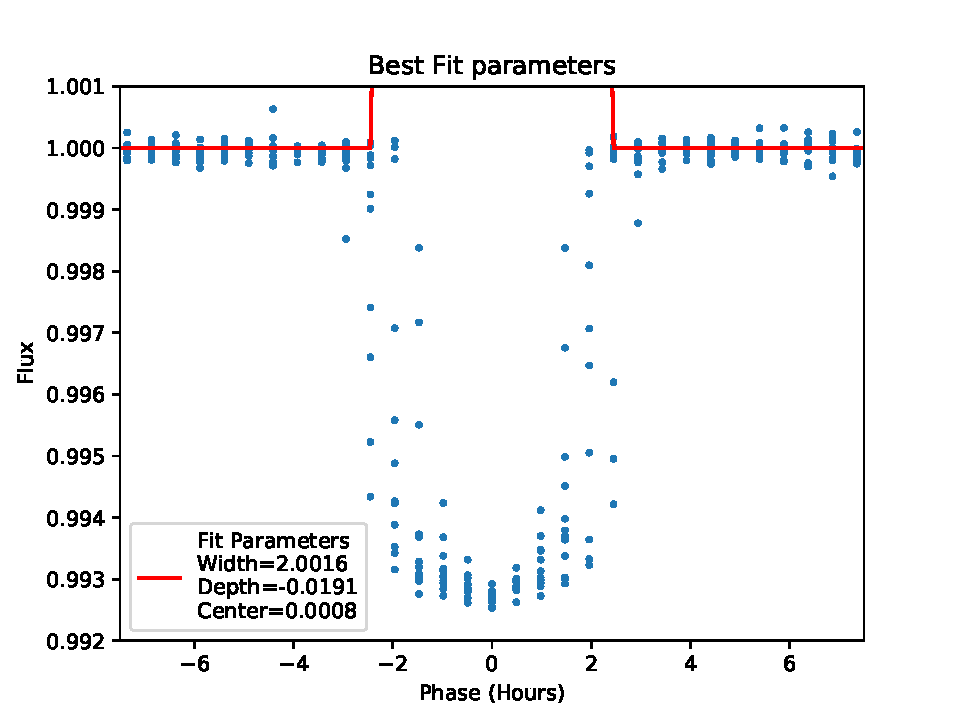
\includegraphics[width=4.5in]{fit.pdf}}
      \caption{Plot of the best fit parameters from the MCMC.}
\end{figure}




\end{document}